\section{Modelado de prote\'\i{}nas por homolog\'{i}a} \label{CM}

Con las herramientas que hemos estado manejando ya estamos preparados para modelar prote\'\i{}nas. 
En este contexto modelar significa hacer una predicci\'{o}n de c\'{o}mo se disponen los \'{a}tomos 
de una prote\'\i{}na conocida su secuencia, con el fin de estudiar su funci\'{o}n molecular, su historia evolutiva o, 
si el modelo es bueno, dise\~nar o muestrear ligandos e incluso calcular sus afinidades \citep{Singh2010}. 
Asimismo este tipo de modelos se usan mucho para estudiar el efecto de mutaciones puntuales \citep{Kellogg2011}.

\begin{itemize}
\item \textbf{PROBLEMA:} disponemos de la secuencia de una prote\'{i}na A y quisi\'{e}ramos conocer, aunque sea de manera aproximada, 
su estructura tridimensional
\item \textbf{SOLUCI\'{O}N PROPUESTA:} estimar coordenadas cartesianas para la mayor\'{i}a de los \'{a}tomos de A, 
en base a la estructura conocida de prote\'{i}nas  similares, que llamamos plantillas, moldes, o \italics{templates}
\end{itemize}

Esta metodolog\'{i}a se llama modelado comparativo o por homolog\'{i}a y se describe en profundidad en este
art\'\i{}culo de \citet{Fiser2003}. %\htmladdnormallink{art\'\i{}culo}{./papers/modeller2003.pdf} 
Hay fundamentalmente dos estrategias, que en general requieren alineamientos entre la secuencia problema y los posibles moldes:
\begin{itemize}

\item Ensamblaje de grandes fragmentos r\'{i}gidos, incluso el plegamiento entero, 
obtenidos de estructuras similares alineadas por medio de su secuencia primaria y secundaria
(\htmladdnormallink{SWISS-MODEL}{http://swissmodel.expasy.org}, 
\htmladdnormallink{IntFOLD}{http://www.reading.ac.uk/bioinf/IntFOLD}, 
\htmladdnormallink{ROBETTA}{http://robetta.bakerlab.org} o 
%\htmladdnormallink{3D-JIGSAW}{http://bmm.cancerresearchuk.org/~3djigsaw} 
\htmladdnormallink{MEDELLER}{http://opig.stats.ox.ac.uk/webapps/medeller/home.pl?app=MEDELLER} para prote\'{i}nas transmembrana).
Esta metodolog\'{i}a corta y pega literalmente fragmentos del esqueleto pept\'{i}dico de estructuras conocidas.

\item Modelado por satisfacci\'{o}n de restricciones (distancias, \'{a}ngulos) moleculares extra\'{i}das 
de bases de datos y estructuras similares alineadas (\htmladdnormallink{MODELLER}{https://salilab.org/modeller/}). 
Este m\'{e}todo, conceptualmente similar a la resoluci\'{o}n por NMR (ver secci\'{o}n \ref{metodosExp}), 
produce un conjunto de estructuras para la secuencia A, 
todas ellas compatibles con las restricciones observadas en los \italics{templates}.

\end{itemize}

El algoritmo gen\'{e}rico de modelado comparativo puede dividirse en varios pasos, ilustrados en la figura \ref{fig:CMflow}:
\begin{itemize}
\item{1.} Identificar por similitud de secuencia dominios $D_{1..d}$ en la prote\'\i{}na $S$ que queremos modelar.
\item{2.} Buscar y alinear estructuras molde $M_{1..m}$ que nos sirvan para modelar uno o m\'{a}s dominios de $S$. 
Cada dominio con al menos un molde es potencialmente modelable.
\item{3.} Para cada dominio $D_{i}$ modelable:
\begin{itemize}
\item{3.1.} Refinar el alineamiento local de cada segmento alineado del molde.
\item{3.2.} Tomar las coordenadas pept\'{i}dicas (o descriptores moleculares) de la estructura molde alineada.
\item{3.3.} Copiar los \htmladdnormallink{rot\'{a}meros}{http://kinemage.biochem.duke.edu/databases/rotamer.php}
de las cadenas laterales de los amino\'{a}cidos conservados en el alineamiento.
\item{3.4.} Modelar los rot\'{a}meros de los residuos que mutan respecto al molde, 
con ayuda de una \htmladdnormallink{biblioteca}{http://dunbrack.fccc.edu/bbdep2010}.
\begin{figure}
\begin{center} 
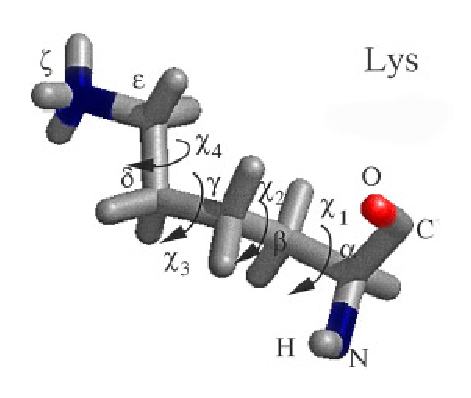
\includegraphics{rotamer}
\caption%[]
{
\'{A}ngulos que definen los rot\'{a}meros de las cadenas laterales.
%figura tomada de \htmladdnormallink{http://bopwww.biologie.uni-freiburg.de}{http://bopwww.biologie.uni-freiburg.de/students/labs/synopsis_jul02/index.html}.
}
\label{fig:rotamer}
\end{center}
\end{figure}
\item{3.4.} A\~nadir los segmentos, normalmente \htmladdnormallink{\italics{loops}}{http://bmm.cancerresearchuk.org/loop}, 
correspondientes a \italics{gaps} en la secuencia alineada del molde.
\item{3.5.} Refinar 1 \'{o} m\'{a}s modelos completos $P_{n}$ con el objeto de eliminar errores obvios de estructura, como impedimentos o choques est\'{e}ricos.
\item{3.6.} Evaluar los modelos $P_{n}$  y estimar su calidad, por medio de aplicaciones como 
\htmladdnormallink{ProQ3}{http://proq3.bioinfo.se},
\htmladdnormallink{Verify3D}{http://services.mbi.ucla.edu/Verify_3D} o 
\htmladdnormallink{FiltRest3D}{http://filtrest3d.genesilico.pl/filtrest3d/index.html}.
\end{itemize}
\end{itemize}

El paso 2 es el m\'{a}s determinante sobre la calidad del modelo y de hecho marca el techo de precisi\'{o}n de la metodolog\'{i}a 
\citep{ContrerasMoreira2005}. Es adem\'{a}s un paso cr\'{i}tico en el sentido de que si el alineamiento $M_{i}$ es malo, 
el modelo resultante ser\'{a} malo, como ya vislumbramos en la secci\'{o}n \ref{3dcons}. Para modelos complicados ser\'{a} 
necesario explorar diferentes combinaciones de moldes y alineamientos para encontrar la mejor soluci\'{o}n. %\citep{Contreras-Moreira2003}.
Si la secuencia problema es multidominio o multim\'{e}rica puede ser necesario modelar su estructura cuaternaria \citep{Tramontano2017}, 
con herramientas especiales como
\htmladdnormallink{BAM}{http://dunbrack.fccc.edu/BAM} o 
\htmladdnormallink{AIDA}{http://ffas.burnham.org/AIDA}.

Con el objeto de explicar en mayor detalle el algoritmo, el siguiente c\'{o}digo implementa los pasos 3.1 y 3.2, quiz\'{a}s
los m\'{a}s fundamentales tras el el paso 2. El programa usa como ejemplo secuencias
y estructuras ya utilizadas en el apartado \ref{3dcons} (\htmladdnormallink{1gd6.pdb}{./files/1gd6.pdb}):
\verbatiminput{code/prog3.3.py}

Como en otros campos de la biolog\'{i}a computacional, el repertorio de software para modelar prote\'{i}nas es muy extenso,
y constantemente incluye nuevas herramientas que sustituyen a otras que envejecen.
Un buen punto de partida para elegir la mejor soluci\'{o}n son los \italics{rankings} que actualiza cada dos a\~nos 
\htmladdnormallink{CASP}{http://predictioncenter.org/index.cgi?page=public_serv}, aunque probablemente los 
programas de modelado preferidos por los usuarios son SWISS-MODEL en la Web y MODELLER como instalable.

\begin{figure}
%\htmlimage{scale=0.5}
\begin{center} 
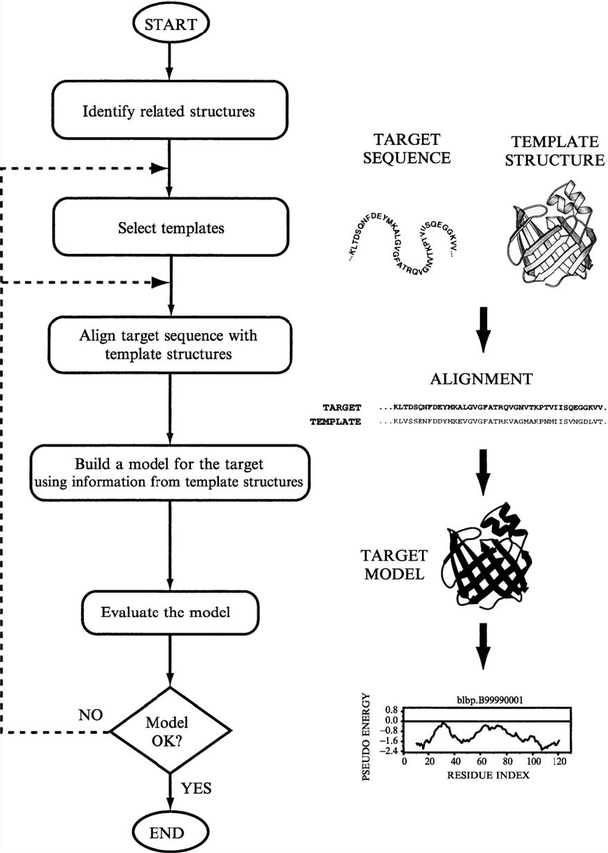
\includegraphics{CMflow}
\caption%[]
{
Algoritmo gen\'{e}rico de modelado comparativo.
Figura tomada de \citet{Fiser2003}. Copyright (2003) Methods in Enzymology.
}
\label{fig:CMflow}
\end{center}
\end{figure}

\begin{figure}
\begin{center} 

\includegraphics{figure_3_contrera_review_final}
\caption%[]
{
Los errores en modelado comparativo se disparan al usar estructuras molde con identidades bajas.
Este comportamiento se observa con diferentes herramientas de modelado, incluyendo SWISS-MODEL.
Figura de \citet{Contreras-Moreira2002b}. 
}
\label{fig:CMbench}
\end{center}
\end{figure}

En la pr\'{a}ctica podemos hacer nuestros modelos por homolog\'{i}a, con la opci\'{o}n de controlar todos los pasos
del procedimiento, por medio del programa \htmladdnormallink{MODELLER}{https://salilab.org/modeller} \citep{Sali1993}, 
disponible sin costo para usuarios acad\'{e}micos. %\verb+/home/bioinfo/bin/modeller8v1/bin/mod8v1+ 
El programa tiene \htmladdnormallink{m\'{u}ltiples posibilidades}{https://salilab.org/modeller/tutorial/}, pero en este ejemplo
nos centramos en el caso m\'{a}s sencillo consistente en hacer un modelo a partir de un s\'{o}lo molde o \italics{template},
estimando su calidad del modelo por medio de la funci\'{o}n DOPE \citep{Shen2006}:
\begin{itemize}

\item Secuencia problema: \htmladdnormallink{FNR}{http://www.expasy.org/uniprot/FNR_ECOLI}, 
regulador transcripcional de \italics{Escherichia coli}.

\item Busca, por ejemplo usando PSI-BLAST, secuencias similares (probablemente hom\'{o}logas)
cuya estructura est\'{e} en el PDB (moldes o \italics{templates}).

\item Para cada uno de los \italics{templates} interesantes sigue estos pasos:
\begin{itemize}

	\item descarga el fichero de coordenadas del \htmladdnormallink{PDB}{http://www.rcsb.org/pdb} 
	y extrae la secuencia S contenida en los campos \verb+ATOM+

	\item alinea la secuencia S de las coordenadas con la secuencia problema (FNR, por ejemplo con 
  \htmladdnormallink{clustal-omega}{https://www.ebi.ac.uk/Tools/msa/clustalo} o usando el mismo alineamiento de BLAST) 
	y crea un archivo con extensi\'{o}n 
	\verb+.ali+ con este formato, donde \verb+structureX+ es el molde, \verb+sequence+ es la secuencia problema o \italics{query} 
	y los dem\'{a}s campos definen el rango de residuos alineados del \italics{template}, y su resoluci\'{o}n:

\begin{verbatim}
C; Alineamiento de muestra en formato PIR
>P1;1PDB
structureX:1PDB:1    :A:106  :A:nombre_template:: 1.90: 
AFVVTDNCIKCKYTDCVEVCPVDCFYEGPNFLVIHPDECIDCALCEPECPAQAIFSEDEVPEDMQEFIQLNAELA
EVWPNITEKKDPLPDAEDWDGVKGKLQHLER*
>P1;query
sequence:query:::::::0.00: 0.00
AYVINDSC--IACGACKPECPVNIIQGS--IYAIDADSCIDCGSCASVCPVGAPNPED-----------------
-------------------------------*
\end{verbatim}

	\item genera un gui\'{o}n o \italics{script} para MODELLER como \verb+guion_nombre_template.py+:

\begin{verbatim}
from modeller.automodel import *   

log.verbose()    
env = environ() 

# 1) directorio donde se encuentran los ficheros con coordenadas de moldes/templates, 
# con extension .pdb,.atm,.ent
env.io.atom_files_directory = './templates/'

# 2) prepara el modelado
a = automodel(env,
              alnfile  = 'alineamiento.ali',  # fichero con el alineamiento
              knowns   = '1PDB',              # nombre del template como aparece en alnfile
              sequence = 'query',             # nombre de secuencia problema como aparece en alnfile
	          assess_methods=(assess.DOPE))      

a.starting_model= 1                           # define cuantos modelos diferentes quieres
a.ending_model  = 2                 
				  
# 3) accion! 
a.make()                  
\end{verbatim}

	\item ahora ejecuta MODELLER (por ejemplo poniendo en el terminal: \verb+$ mod9v8 guion_template.py+ y al terminar revisa 
	\verb+guion_nombre_template.log+ para comprobar la evaluaci\'{o}n emp\'{i}rica del modelo o modelos obtenidos

\end{itemize}
\end{itemize}


%%%%%%%%%%%%%%%%%%%%%%%%%%%%%%%%%%%%%%%%%%%%%%%%%%%%%%%%%%%%%%%%%%%%%%%%%%%%%%%
%%%%%%%%%%%%%%%%%%%%%%%%%%%%%%%%%%%%%%%%%%%%%%%%%%%%%%%%%%%%%%%%%%%%%%%%%%%%%%%


\section{Modelado de prote\'\i{}nas \italics{ab initio}} \label{abinitio}

Hablamos de protocolos \italics{ab initio} cuando tratamos de modelar
el plegamiento de un polip\'{e}ptido solamente a partir de su secuencia y de la f\'\i{}sica  \citep{Baker2001}. 
Sin embargo, los m\'{e}todos de este tipo
m\'{a}s exitosos hasta la fecha reconstruyen la estructura terciaria a base de peque\~{n}os fragmentos cortados 
de estructuras conocidas y seleccionados por similitud de secuencia. 

El mejor ejemplo es el algoritmo Rosetta \citep{Simons1997}, implementado en el servidor web 
\htmladdnormallink{ROBETTA}{http://robetta.bakerlab.org}, 
que permite modelar secuencias cortas cuando no hay moldes que alineen con la secuencia problema, 
ni siquiera por \italics{fold recognition} (ver secci\'{o}n \ref{FRsection}). 
Usa fragmentos de 9 amino\'{a}cidos de longitud. En este caso podemos definir el problema tipo de esta manera:

\begin{itemize}
\item \textbf{PROBLEMA:} disponemos de la secuencia de una prote\'{i}na A y quisi\'{e}ramos conocer, aunque esa de manera aproximada, su estructura tridimensional
\item \textbf{SOLUCI\'{O}N PROPUESTA:} combinar fragmentos tomados de estructuras del PDB, generar conformaciones alternativas y seleccionar las mejores
\end{itemize}

\begin{figure}
\begin{center} 
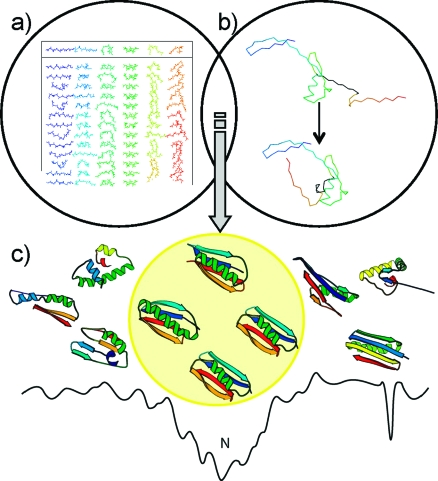
\includegraphics{rosetta}
\caption%[]
{
Resumen del protocolo Rosetta, tomado de \citet{Kaufmann2010}.
A) Se seleccionan de una biblioteca los fragmentos con secuencias mas parecidas a los $K$-meros de la secuencia problema ($K=9$).
B) Combinaci\'{o}n de fragmentos solapantes para generar muchas conformaciones alternativas.
C) Optimizaci\'{o}n de conformaciones con funciones que eval\'{u}an interacciones no locales. 
Copyright (2010) Biochemistry.
}
\label{fig:Rosetta}
\end{center}
\end{figure}

Este tipo de algoritmos requieren tener precalculada una biblioteca de fragmentos de longitud $K$ de estructura conocida,
funciones para seleccionar los mejores fragmentos para cada $K$-mero de la secuencia problema,
funciones de evaluaci\'{o}n que permitan descubrir conformaciones que se parezcan a las nativas, 
y muchos recursos computacionales, dado que todos estos pasos son costosos.
Otro algoritmo que funciona tanto para \italics{fold recognition} como para modelado \italics{ab initio} es 
\htmladdnormallink{I-TASSER}{http://zhanglab.ccmb.med.umich.edu/I-TASSER}:

\begin{figure}
\begin{center} 
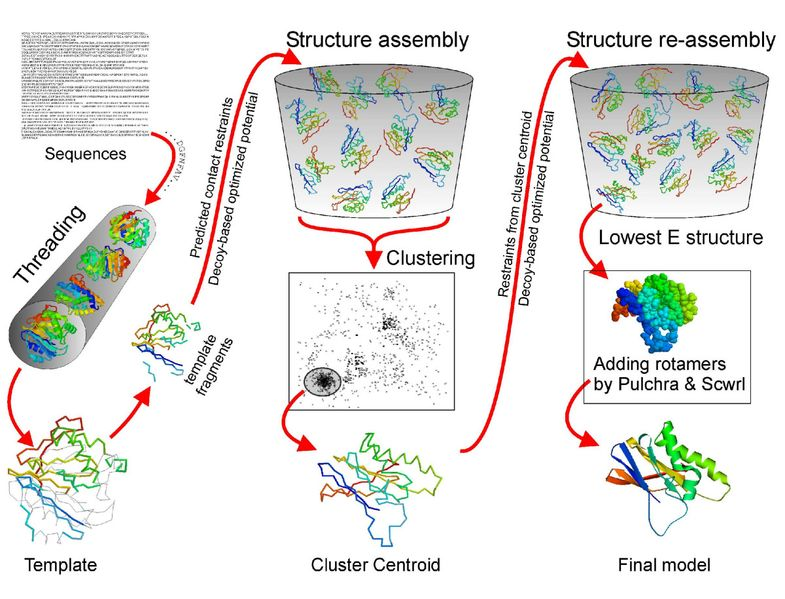
\includegraphics{ITASSER}
\caption%[]
{
Resumen del protocolo TASSER. 
Figura de \citet{Wu2007}, reproducida con permiso de los autores.
}
\label{fig:ITASSER}
\end{center}
\end{figure}
